\documentclass[9pt]{beamer}
\usetheme{default}
\usepackage{datetime}
\usepackage{adjustbox}
\usepackage{amsmath}
\usepackage{mathtools}
\usepackage{listings}
\usepackage{hyperref}
\usepackage{amsmath}
\usepackage{amssymb}
\usepackage{multicol}
\usepackage{algorithmic, algorithm}
\usepackage{booktabs} % For prettier tables
\usepackage{graphicx}

\newdate{date}{26}{01}{2024}

\title{\Large Verification of ACAS-Xu benchmark using Alpha Beta Crown and Nnenum}

\author{\mbox{Amalia Duma Diana} \and \mbox{Răzvan Maciovan Alexandru} \and \mbox{Luca Mitroi} \and \mbox{Vlad Petcu} \and \mbox{Vlad Țîrcomnicu} \and}

\institute{West University of Timi\c soara\\Faculty of Mathematics and Informatics

Master Study Program: Software Engineering

\bigskip

Scientific Coordinator: Mădălina Erașcu}

\date{\small{\displaydate{date}}
	
\bigskip


%\titlegraphic{
\begin{center}
\includegraphics[height=1.0cm]{UVTlogo}
\end{center}
	\centering{
		
		%\includegraphics[height=1.0cm]{DKlogo} \hspace{0.9cm}
		%\includegraphics[height=0.8cm]{OeAWLogo} \hspace{0.9cm}
		%\includegraphics[height=1.0cm]{NCSUlogo}
	}
%}
}

% \AtBeginSubsection[]
% {
%   \begin{frame}[t]<beamer>{Overview}
%     \tableofcontents[currentsection,currentsubsection]
%   \end{frame}
% }

\begin{document}

\begin{frame}[t]
  \titlepage
\end{frame}

 
\section{Motivation and Problem Specification}
\begin{frame}{Motivation and Problem Specification}
  The ACAS-Xu system is designed to enhance airspace safety by providing resolution advisories. We aimed to verify the reliability of ACAS-Xu neural networks using verification tools, namely Alpha-Beta-CROWN and Nnenum.
\end{frame}

\section{Dataset Description}
\begin{frame}{Dataset Description}
  The ACAS-Xu dataset contains inputs representing sensor readings and advisories for unmanned aircraft. We then mix the time until loss of vertical separation (\(\tau\)) and the previous advisory (\(a_{\text{prev}}\)) to get five outputs: Clear-of-Conflict (COC), weak/strong right, weak/strong left.
  \begin{figure}[ht]
    \centering
    \begin{minipage}[b]{0.45\linewidth}
        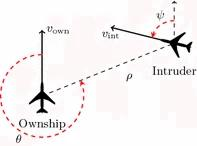
\includegraphics[width=\linewidth]{Figures/acasxu_geometry.jpg}
        \caption{Geometry of ACAS Xu horizontal logic table \cite{katz2017reluplex}}
        \label{fig:acasxu-geometry}
    \end{minipage}
    \hfill
    \begin{minipage}[b]{0.45\linewidth}
        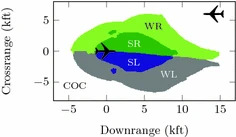
\includegraphics[width=\linewidth]{Figures/acasxu_advisories.jpg}
        \caption{Advisories for a head-on encounter with \(a_{\text{prev}}\) = Clear of Conflict and \(\tau\) = os \cite{katz2017reluplex}}
        \label{fig:acasxu-advisories}
    \end{minipage}
\end{figure}
\end{frame}

\section{Tools Used and Challenges}
\begin{frame}{Tools Used and Challenges}

  % Alpha-Beta-CROWN, a tool for formal verification, requires conda in order to compile. Installation challenges included environment setup and dependencies management.
  % A neural network verifier based on an efficient linear bound propagation framework.
\begin{block}{Alpha-Beta-CROWN}
\vspace{0.1cm}
  A neural network verifier based on an efficient linear bound propagation framework.
\end{block}
  
\begin{itemize}
    \item Prerequisites: Conda
    \vspace{0.2cm}
\end{itemize}


Setting up the tool involved a two-step process: installing Miniconda, which was straightforward, and then the tool itself, which presented complications. 

\vspace{0.15cm}

The tool's installation required resolving errors related to the conda environment configuration and manually retrieving essential files due to permission issues.
\end{frame}

\begin{frame}{Tools Used and Challenges}

\begin{block}{Nnenum}
\vspace{0.1cm}
  A neural network verifier that relies on multiple levels of abstraction to achieve high performance verification of ReLU networks without sacrificing completeness.
\end{block}

\begin{itemize}
    \item Prerequisites: Docker
    \vspace{0.2cm}

\end{itemize}

Following the steps outlined in the GitHub repository's "Getting started" section, including cloning the repository and executing two commands in the docker file, ensured a straightforward installation without any errors or unexpected behavior.

% Nnenum, another verification tool, offers a docker environment that simplifies the setup. This not only simplifies the installation process, but it also eliminates all dependencies challenges thanks to the docker container properties.
  %TODO: Provide examples of output interpretation challenges.
\end{frame}

\section{Experimental Results}
\begin{frame}{Experimental Results}

The verification process involved evaluating 10 properties on 45 DNNs. The first four properties were assessed across all networks, while the rest were checked on a single network, following the original authors' approach. A consistent timeout of 116 seconds was applied to each property evaluation.

\vspace{0.6cm}

The final verified accuracy stands at approximately 74.73\%.

\begin{table}[h!]
\centering
\footnotesize
\begin{tabular}{ccccccc}
\toprule
Tool & Verified & Falsified & Penalty & Score & Avg. time & Max time \\
\midrule
alpha-beta-CROWN & 139 & 47 & 0 & 1860 & 2.58 & 69.08 \\
nnenum & 139 & 47 & 0 & 1860 & 2.3 & 61.58 \\
\bottomrule
\end{tabular}
\caption{Benchmark 2023-ACAS-Xu}
\label{table:res1}
\end{table}
\end{frame}

\begin{frame}{Experimental Results}

\begin{table}[h!]
\centering
\footnotesize
\begin{tabular}{lllr}
\toprule
ONNX & VNN-LIB & Result & Time (seconds) \\
\midrule
onnx/ACASXU\_run2a\_1\_1\_batch\_2000.onnx & vnnlib/prop\_1.vnnlib & unsat & 5.5214 \\
onnx/ACASXU\_run2a\_1\_9\_batch\_2000.onnx & vnnlib/prop\_7.vnnlib & sat & 0.355 \\
\bottomrule
\end{tabular}
\caption{Example of results for Alpha-Beta-CROWN}
\label{table:ex_nnenum_abc}
\end{table}

\begin{table}[h!]
\centering
\footnotesize
\begin{tabular}{lllr}
\toprule
ONNX & VNN-LIB & Result & Time (seconds) \\
\midrule
onnx/ACASXU\_run2a\_3\_4\_batch\_2000.onnx & vnnlib/prop\_1.vnnlib & holds & 1.46 \\
onnx/ACASXU\_run2a\_1\_9\_batch\_2000.onnx & vnnlib/prop\_3.vnnlib & violated & 0.93 \\
\bottomrule
\end{tabular}
\caption{Example of results for Nnenum}
\label{table:ex_nnenum}
\end{table}
\end{frame}

\section{Conclusion and Future Work}
\begin{frame}{Discussion and Conclusions}
  Our investigation shows the importance of formal verification in ensuring the safety of systems affecting real life scenarios like ACAS-Xu.

  \vspace{0.6cm}

  This study aimed to replicate results from VNN-COMP 2023 using alpha-beta-CROWN and nnenum as the neural network verifiers. While the tools produced identical results, alpha-beta-CROWN stood out by the absence of the timeout penalty that was applied in the competition

  \vspace{0.6cm}

  The verification process maintained consistency with competition parameters and utilized files sourced directly from the official GitHub repository.

\end{frame}


\begin{frame}{References}
    
\bibliography{Bibliography/refs}
\bibliographystyle{plain}
\end{frame}

\end{document}



